\documentclass[12pt]{article}
\usepackage{graphicx}
\usepackage[colorlinks=true, urlcolor=black]{hyperref}
\title{Sistema Acad\'emico Fractal\\Manual del Padre o Apoderado}
%\author{Edson A. Ticona Zegarra}
\date{Abril 2019}

\renewcommand{\figurename}{Figura}
\begin{document}
\maketitle

\section{Login}
Al ingresar a la direcci\'on \url{www.fractal.edu.pe:9000/asistencias/} 
\footnote{Todas las im\'agenes contienen otra direcci\'on (URL) que no debe ser tomada en cuenta.}
se muestra la p\'agina de la figura~\ref{fig:login}.
Ingresar con su usuario y contrase\~na. Las credenciales de acceso son estrictamente de uso personal y
se recomienda extremo cuidado en no usar contrase\~nas simples.
\begin{figure}[ht]
  \centering
  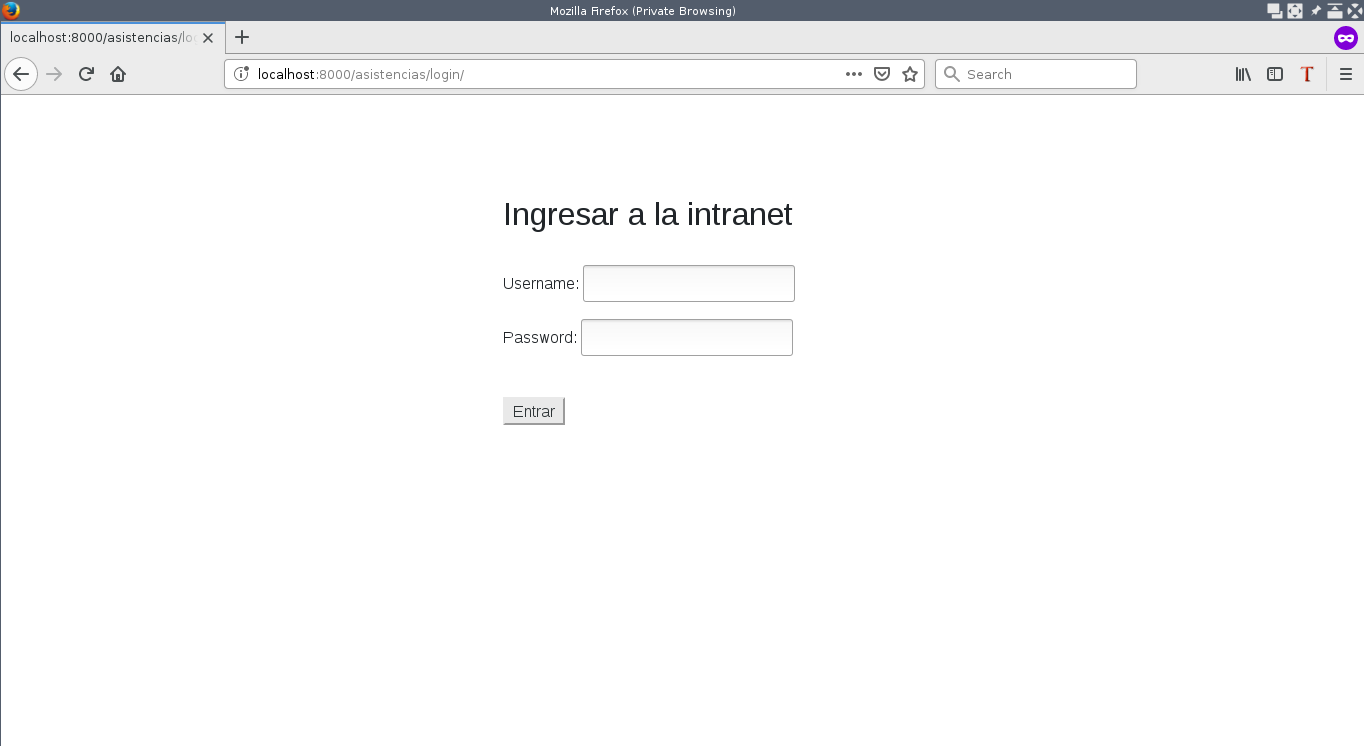
\includegraphics[width=0.8\textwidth]{images/login.png}
  \caption{P\'agina de login}
  \label{fig:login}
\end{figure}

\section{Asistencias}
Una vez logeado, la primera p\'agina en mostrarse al usuario es aquella que permite ver las asistencias.
En la parte superior se puede ver la barra de navegaci\'on con los menus
disponibles al lado izquierdo; al lado derecho, se muestra el nombre del padre o apoderado y
la opci\'on de Salir.
La figura~\ref{fig:asistencias} muestra un ejemplo. En la parte inferior se puede ver la leyenda. 
Rojo es una falta, amarillo una tardanza y verde una asistencia.
\begin{figure}[ht]
  \centering
  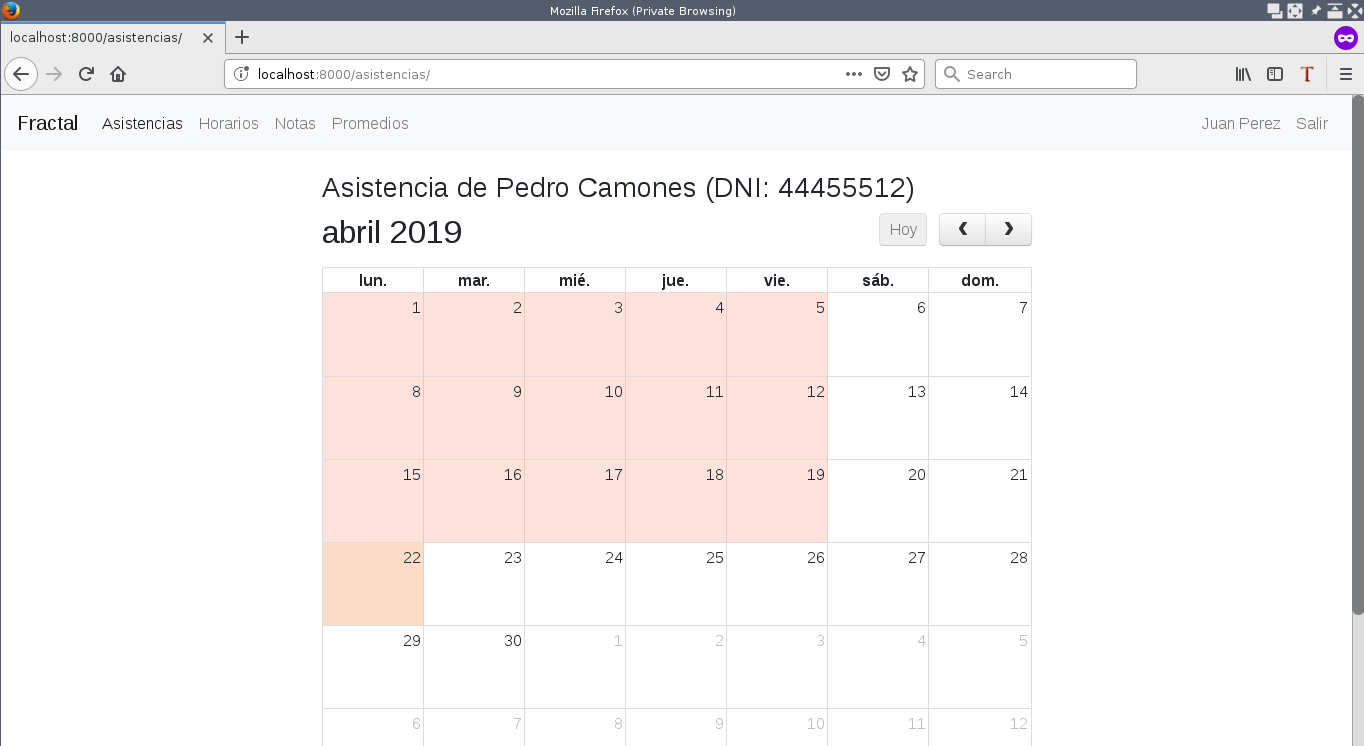
\includegraphics[width=0.8\textwidth]{images/apoderado1.png}
  \caption{Asistencias}
  \label{fig:asistencias}
\end{figure}

\newpage
\section{Horarios}
Al hacer click en el men\'u de horarios, se muestra los horarios del estudiante, tal como se
aprecia en la figura~\ref{fig:horarios}.
\begin{figure}[ht]
  \centering
  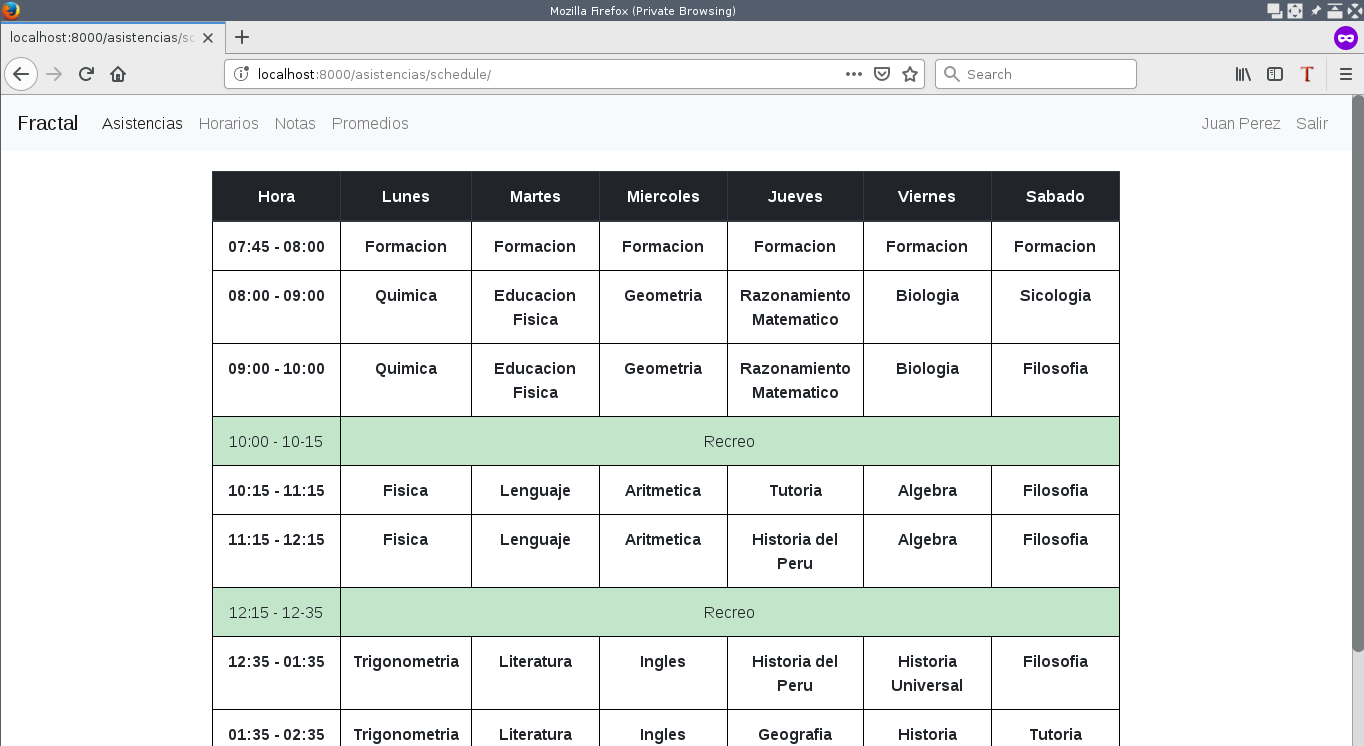
\includegraphics[width=0.8\textwidth]{images/apoderado2.png}
  \caption{Horarios}
  \label{fig:horarios}
\end{figure}

\newpage
\section{Notas}
Al hacer click en el men\'u de notas, se muestran las notas diarias del estudiante. 
Se comienza con el nombre del docente, el grado y secci\'on. Luego un campo fecha, que permite
cambiar la fecha de las notas.
Finalmente, se muestra la lista de los cursos con sus respectivas notas diarias.
\begin{figure}[ht]
  \centering
  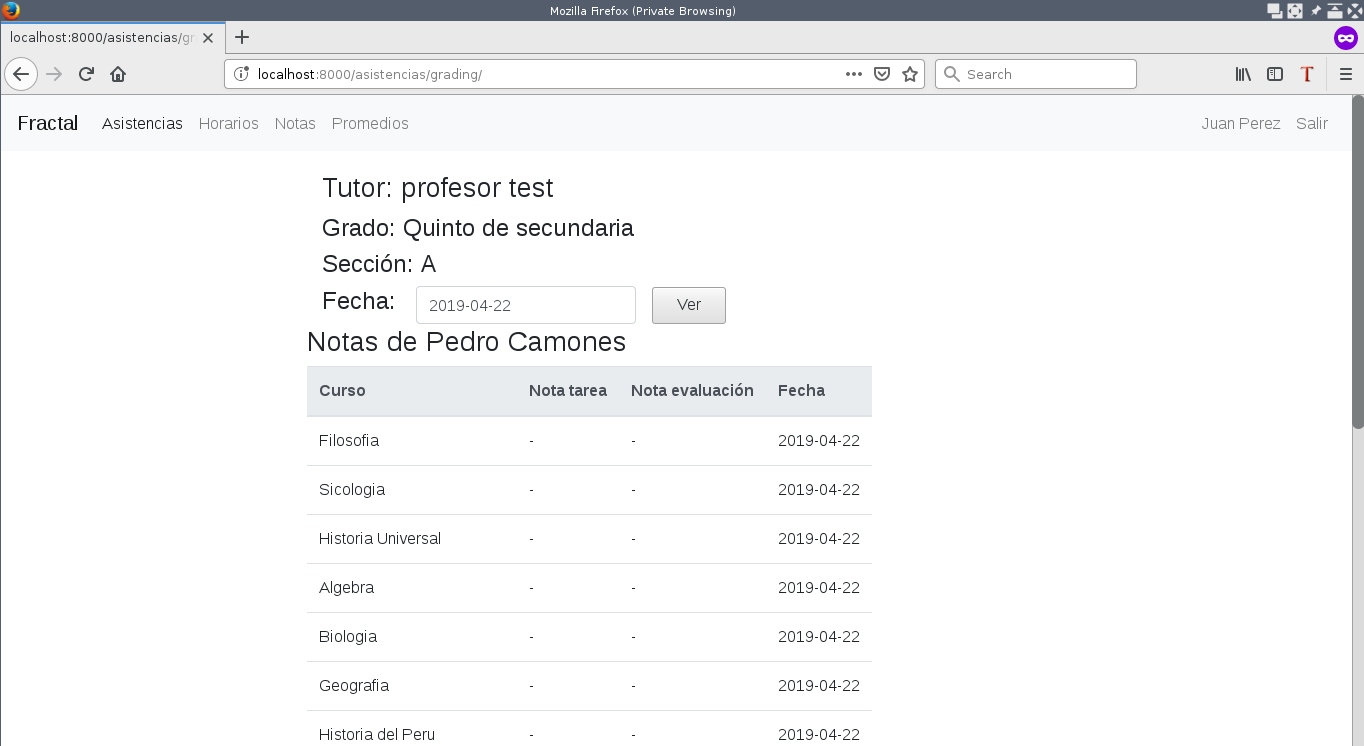
\includegraphics[width=0.8\textwidth]{images/apoderado3.png}
  \caption{Notas}
  \label{fig:notas}
\end{figure}

Si se quiere ver otra fecha, basta con ingresar otra fecha en el campo adecuado y hacer click en 
Ver, como se muestra en la figura~\ref{fig:notas_cal}.
Un gui\'on en las columnas ``Nota tarea'' y ``Nota evaluaci\'on'' indica que el docente a\'un 
no ingres\'o la nota.
\begin{figure}[ht]
  \centering
  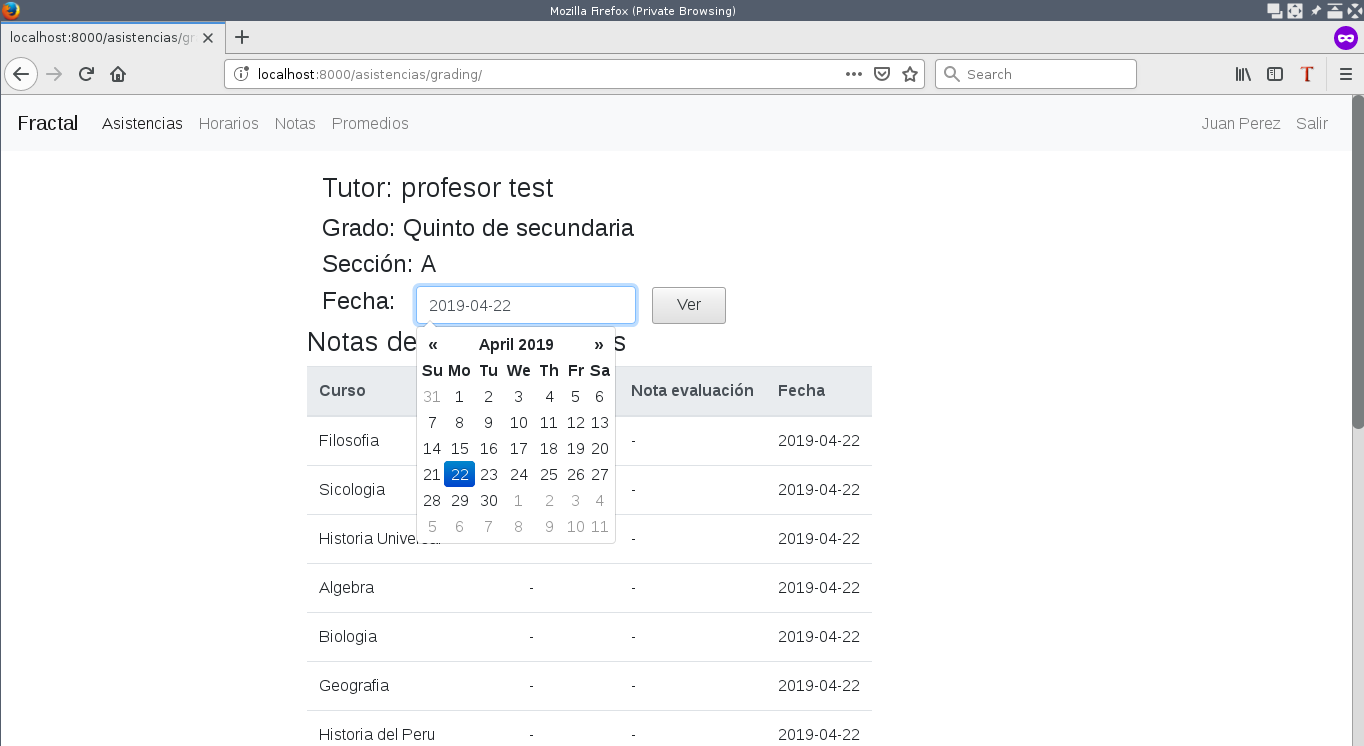
\includegraphics[width=0.8\textwidth]{images/apoderado4.png}
  \caption{Notas}
  \label{fig:notas_cal}
\end{figure}

\newpage
\section{Promedios}
Al hacer click en el men\'u de promedios, se muestran los promedios mensales del estudiante. 
Se comienza con el nombre del docente, el grado y secci\'on. Luego un campo periodo, que permite
cambiar el periodo de las notas.
Finalmente, se muestra la lista de los cursos con sus respectivos promedios por periodo.
\begin{figure}[ht]
  \centering
  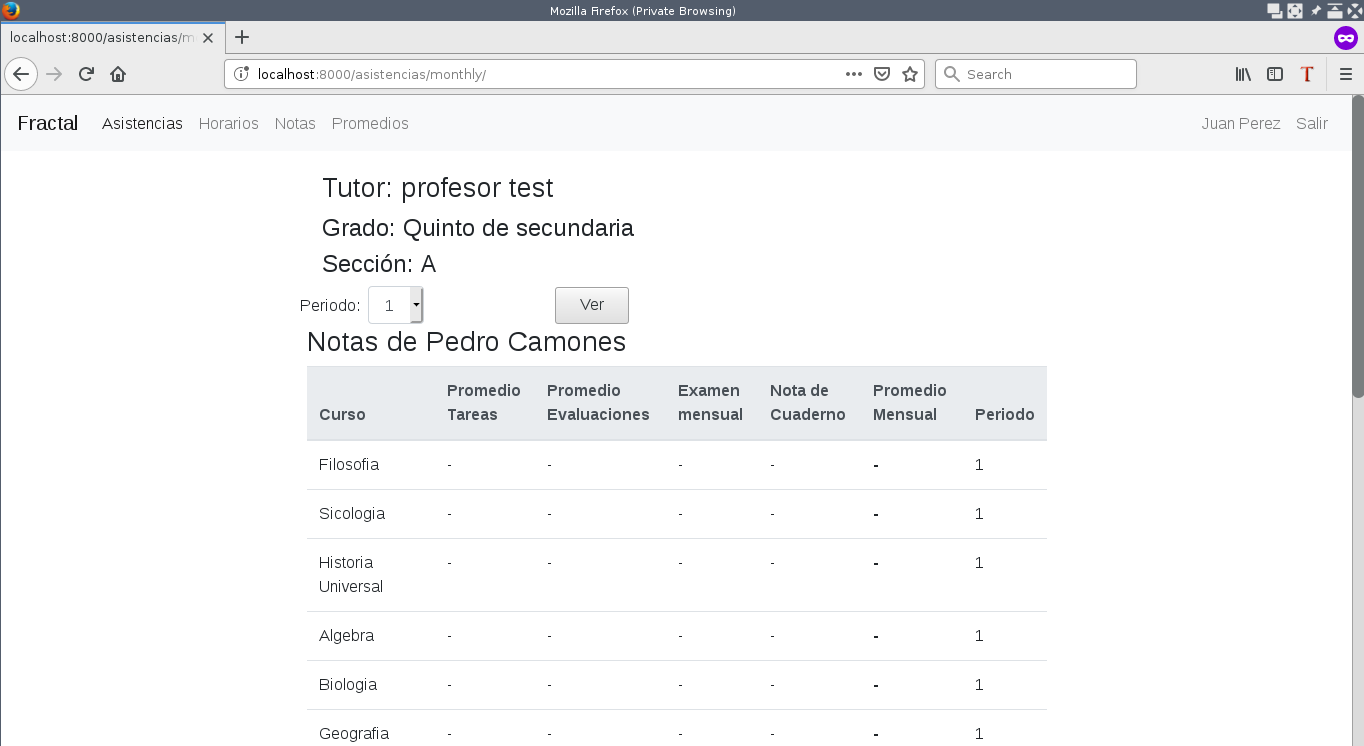
\includegraphics[width=0.8\textwidth]{images/apoderado5.png}
  \caption{Promedios}
  \label{fig:promedios}
\end{figure}
Si se quiere ver otro periodo, basta con seleccionar otro periodo en el campo adecuado y hacer click en 
Ver, como se muestra en la figura~\ref{fig:promedios_select}. Note que la \'ultima columna indica el
periodo al que pertenece la nota.
Un gui\'on en cualquiera de las columnas indica que el docente a\'un 
no ingreso la nota.
En el caso del promedio mensual, se mostrar\'a un gui\'on hasta que el docente haya ingresado todas las
notas necesarias para calcular el promedio.
\begin{figure}[ht]
  \centering
  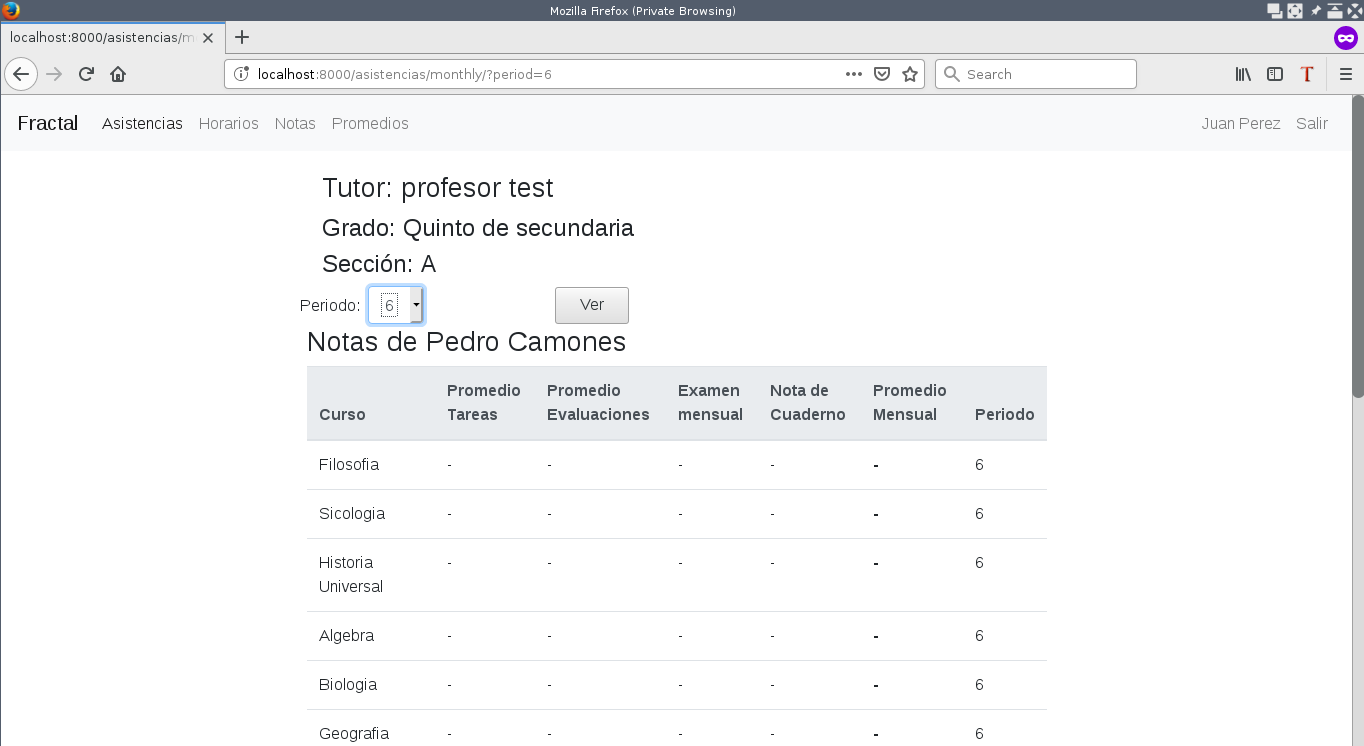
\includegraphics[width=0.8\textwidth]{images/apoderado6.png}
  \caption{Promedios}
  \label{fig:promedios_select}
\end{figure}
\end{document}
